\emph{
    Ejecute y explique la funci\'on del siguiente c\'odigo en Octave. 
    Incluya una gr\'afica en la que la longitud de la variable k sea mayor a 1000. 
    (Puede modificar el programa...) En la gr\'afica observara un esbozo de la 
    trayectoria de un proceso de ramificaci\'on continuo (en una escala distinta...).
    \texttt{
        \lstinputlisting[caption=]{tarea3/problema3_4/binaryGW.R}
    }
}

\afterstatement\par\null

\begin{center}
    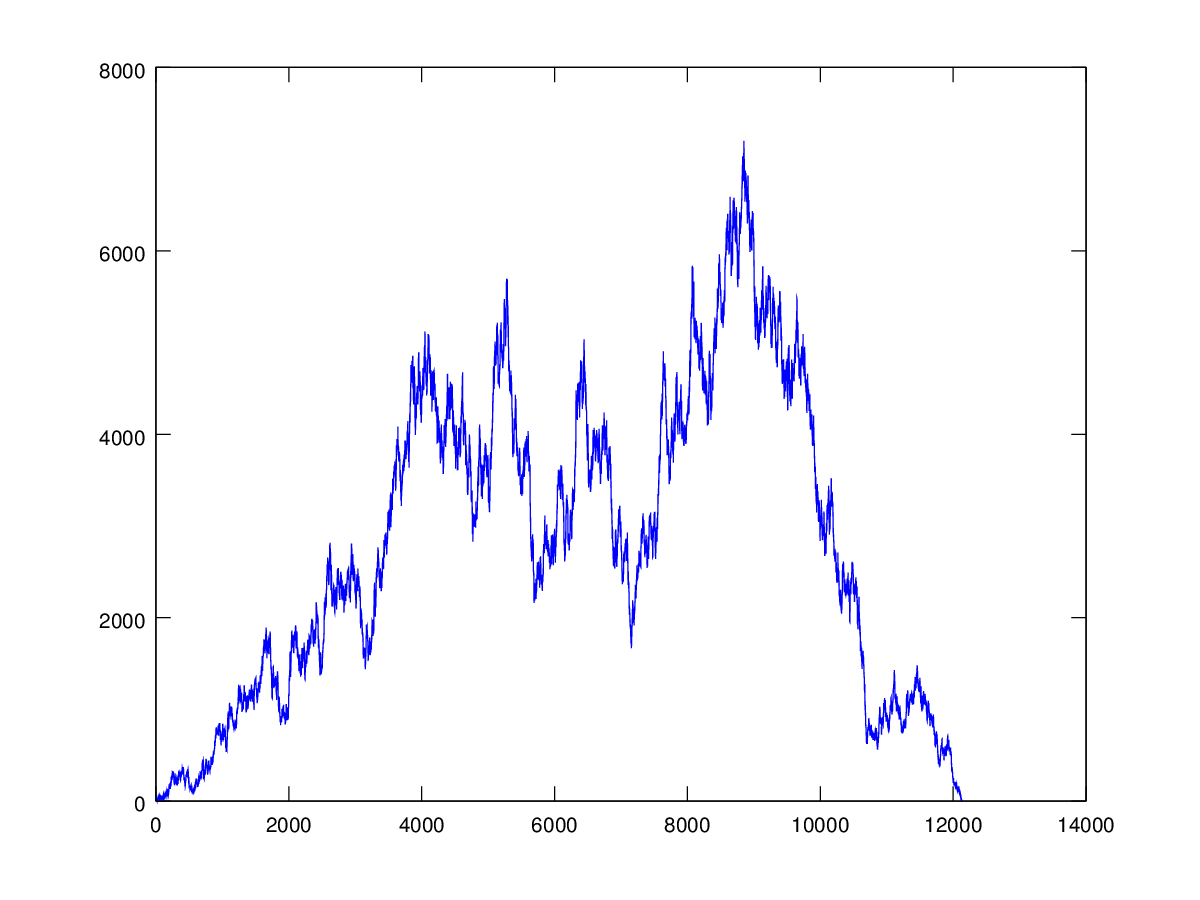
\includegraphics[width=8cm]{tarea3/problema3_4/galtonWatson.PNG}
    
    Gr\'afica de una ejecuci\'on del proceso de extinci\'on de Galton-Watson 
    Par\'ametros: 10 individuos
    La probabilidad de que un individuo tenga $2$ hijos es $\frac{1}{2}$
    La probabilidad de que un individuo tenga $0$ hijos es $\frac{1}{2}$.
\end{center}